\section[Introdução]{Introdução}

O projeto de desenvolvimento do dashboard para a Polícia Civil foi realizado durante o semestre de 2025/1, com reuniões regulares nas terças-feiras e quintas-feiras, das 17h30 às 19h00, com o objetivo de atender à necessidade de centralizar e analisar dados operacionais e administrativos de maneira eficiente. Este projeto visa criar uma solução para a visualização de dados em tempo real, permitindo uma gestão mais ágil e eficaz para os gestores da Polícia Civil, como o Chefe de Polícia e os Diretores de Departamentos. \\
A proposta surge da necessidade de integrar dados de diferentes departamentos, divisões e delegacias da Polícia Civil, oferecendo uma visão abrangente das operações e desempenho dos agentes. Atualmente, há uma dificuldade na visualização e interpretação desses dados, impactando a rapidez nas tomadas de decisão. Com a criação deste dashboard, será possível analisar indicadores como produtividade, número de ocorrências, tempo de resolução e desempenho dos agentes, melhorando a eficácia das ações e intervenções da polícia. \\
O sistema será acessível por navegadores web e dispositivos móveis, oferecendo flexibilidade e mobilidade aos gestores. O dashboard terá funcionalidades como visualizações gráficas dinâmicas, filtros personalizados e alertas em tempo real, proporcionando uma ferramenta essencial para a gestão estratégica e operacional da Polícia Civil. \\
O projeto será conduzido de acordo com a metodologia ágil, com encontros periódicos com os stakeholders, para garantir alinhamento contínuo entre as expectativas do cliente e os resultados alcançados. A seguir, a duração detalhada de cada Sprint será apresentada, ilustrando o planejamento do trabalho e os marcos atingidos ao longo do projeto.

\begin{table}[H]
    \centering
    \caption{Período de cada Sprint - AGES II}
    \begin{tabular}{|c|c|}
        \hline
        \textbf{Sprints} & \textbf{Período} \\
        \hline
        0 & 08/03/2024 a 22/03/2024\\
        1 & 22/03/2024 a 19/04/2024 \\
        2 & 119/04/2024 a 10/05/2024 \\
        3 & 10/05/2024 a 31/05/2024 \\
        4 & 31/05/2024 a 21/06/2024 \\
        \hline
    \end{tabular}
\end{table}

Este projeto foi desenvolvido sob a orientação do professor Dilnei Venturini. A equipe responsável pelo projeto ’Dashboard para a Polícia Civil’ está retratada na Figura 2.


\begin{figure}[H]
    \centering
    \small
    \caption{Time responsável pelo projeto}
    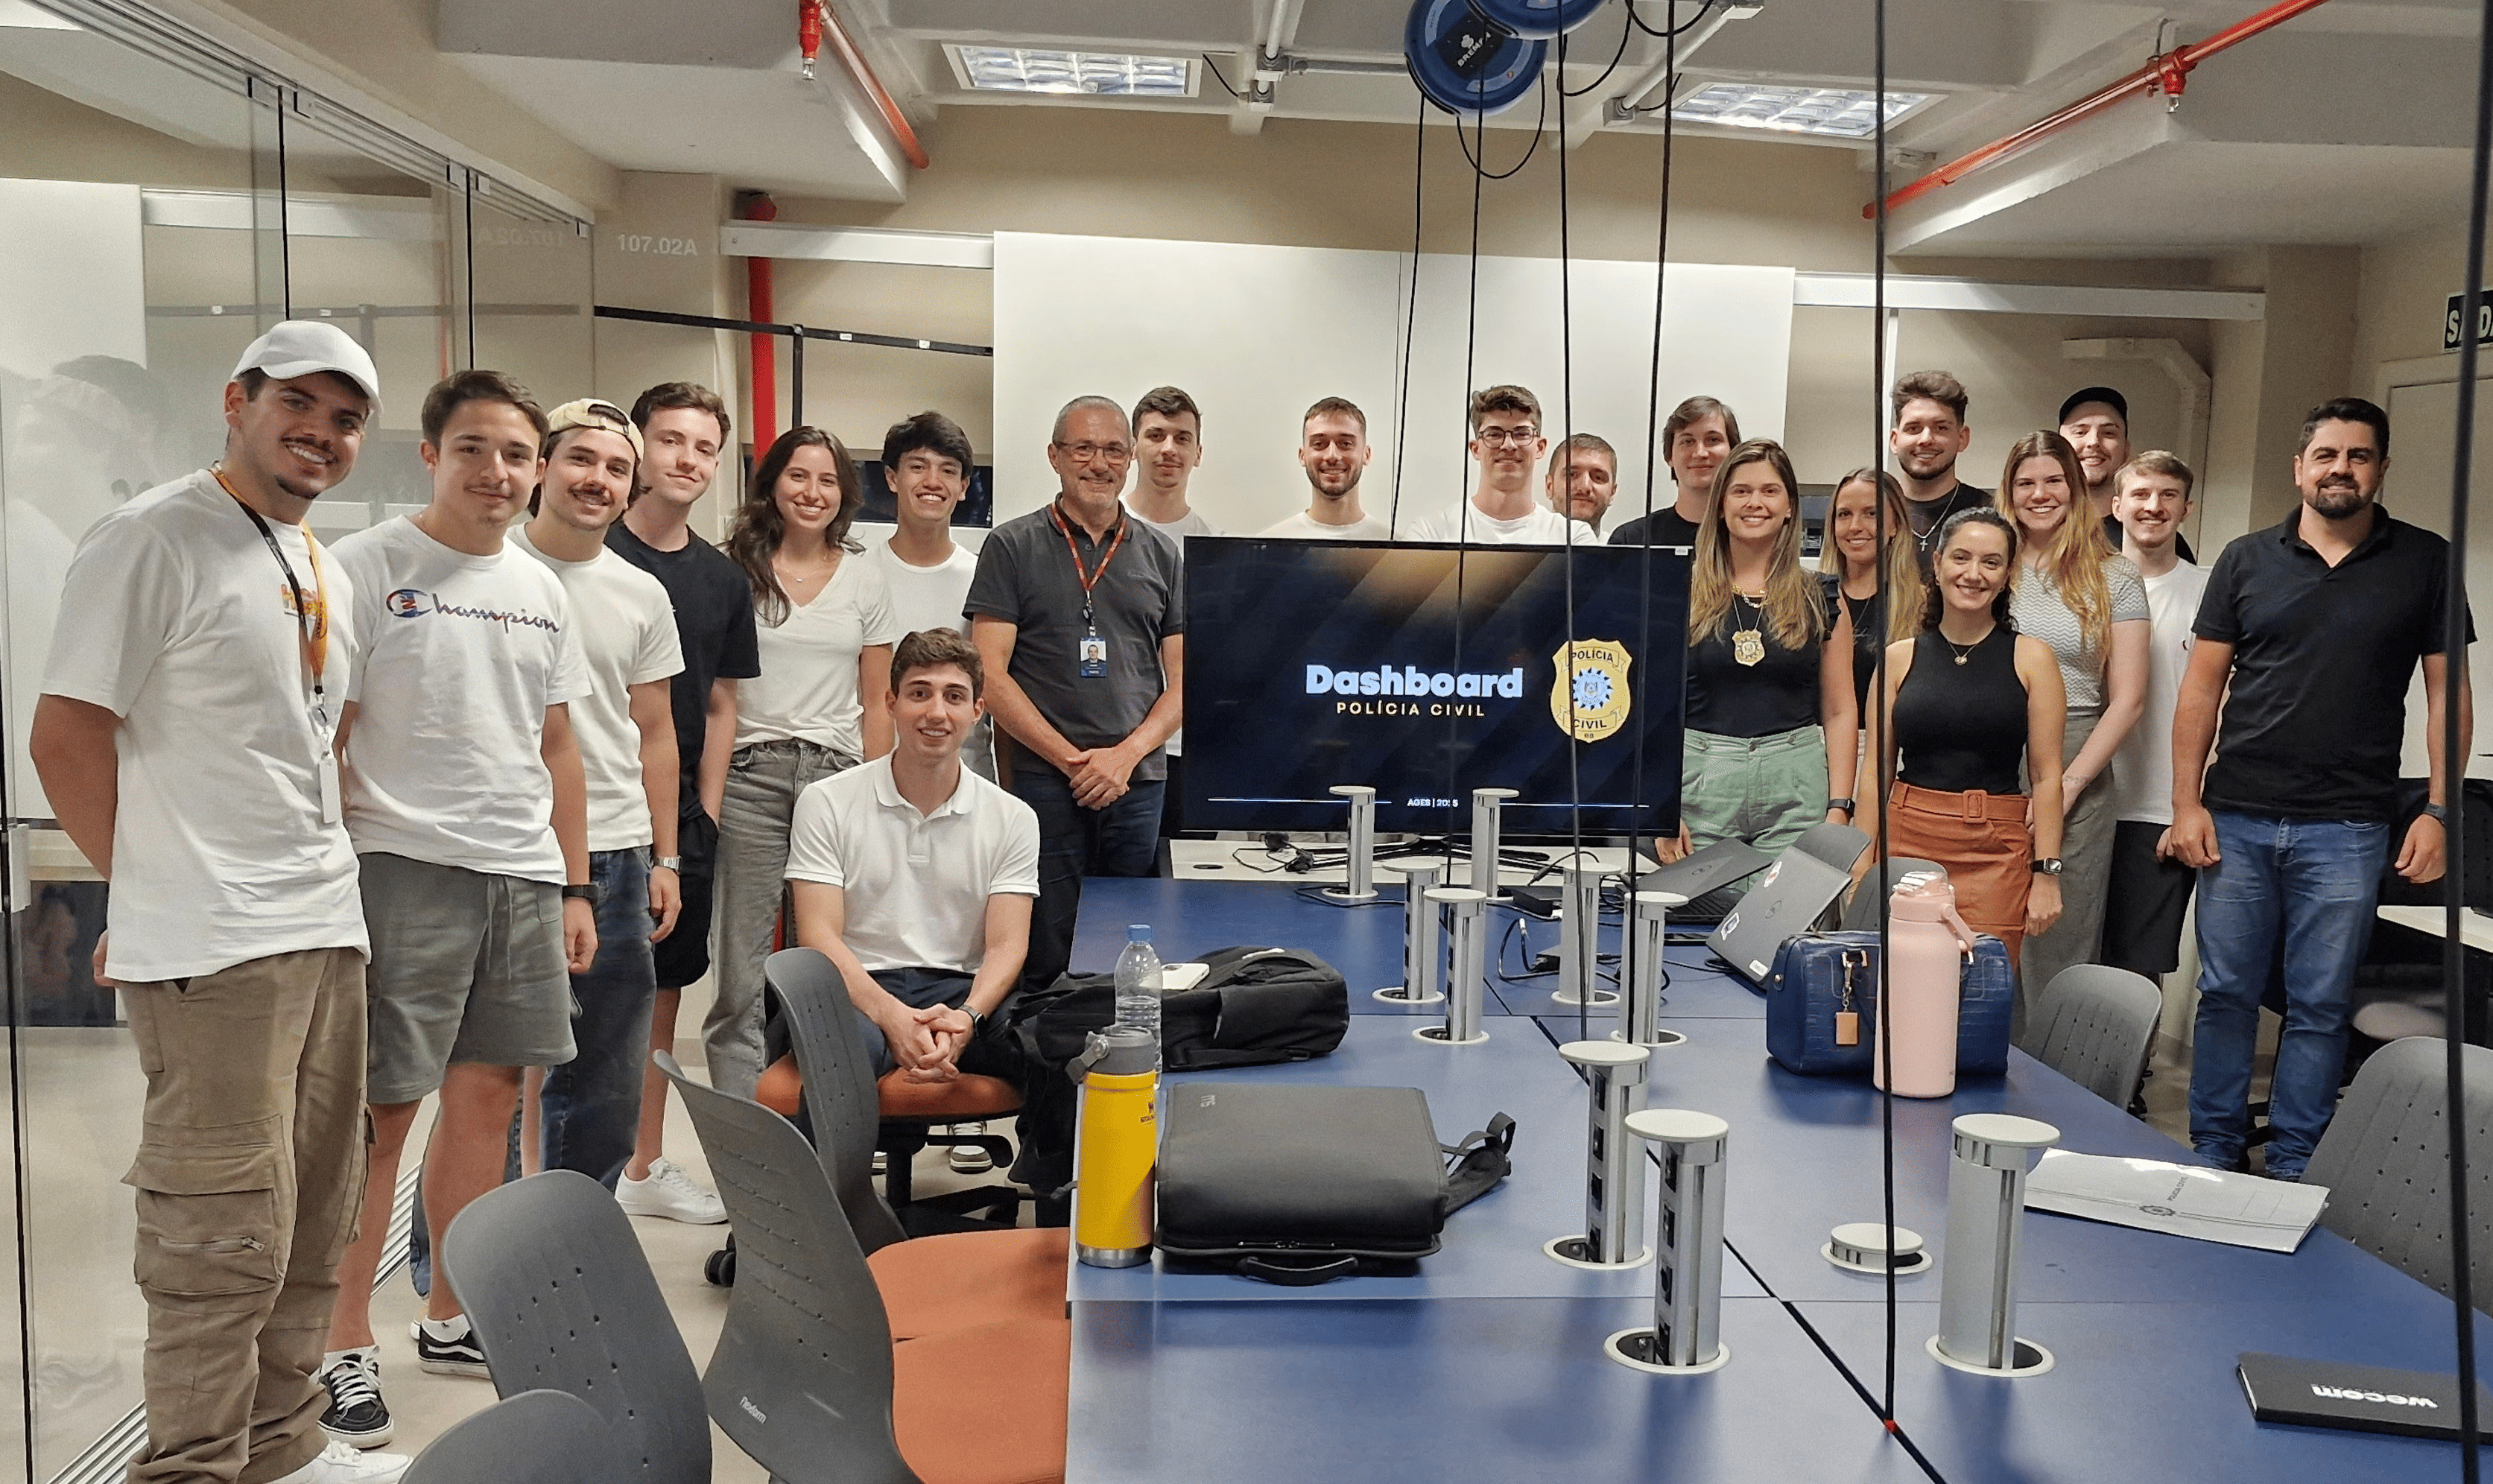
\includegraphics[width=1\linewidth]{conteudo/3 - ages II/conteudo/figures/equipe-policia-civil.png}
    \textit{Fonte: Wiki do Projeto}
    \label{fig:projeto-time}
\end{figure}